\section{Introduction}
\label{sec:intro}


% To understand natural language questions and automatically find
% accurate answers (QA) is a core \abr{nlp} task.


Factoid question answering ~\cite[\abr{qa}]{wang2006survey,iyyer2014neural, gardner2019question}, which asks precise facts about entities, 
is a long-standing problem in
natural language processing (\abr{nlp}) and information retrieval (\abr{ir}).
%
A preponderance of knowledge graphs (\abr{kg})
such as Freebase~\cite{bollacker2008freebase}, \dbpedia{}~\cite{mendes2011dbpedia}, 
\abr{yago}~\cite{suchanek2007yago}, and Wikidata~\cite{vrandevcic2014wikidata}
have been fruitfully applied to factoid \abr{qa} over knowledge
graphs (\abr{kgqa})~\cite[inter alia]{bordes2014question, dong-etal-2015-question}. 
%is a core \abr{nlp} task.
A typical \abr{kgqa} task is to search for entities or
entity attributes from a \abr{kg}.
%
For example, given the question ``who was the last emperor of China'',
the model identifies emperors of China and then reasons to determine
which emperor is the last and find the answer, \candidate{Puyi}.




\kgqa{} approaches solve the problem by
either parsing questions into executable logical
form~\cite{cai2013large, kwiatkowski2013scaling} or aligning questions
to sub-structures of a knowledge graph~\cite{yao2014information,
  yih2015semantic}.
%
Whether these approaches work depends on the underlying \abr{kg}: they
are effective when the knowledge graphs have high coverage 
on the relations targeted by the questions, which is often not the case:
%
%%CZ Oct 13: I slightly change this sentence 
%However, most only have sparse coverage of relations.
Obtaining relation data is costly and requires expert knowledge 
 to design the relation schema and type
 systems~\cite{Paulheim2018HowMI}.
 %
For example, Google's Knowledge Vault has 570M entities, fourteen times more
than Freebase, but only has 35K relation types: similar to
Freebase~\cite{knowledgevalut, bollacker2008freebase}.


In the real world, human knowledge is often tested through
competitions like Quizbowl~\cite{boyd-graber-12} or
\jeopardy{}~\cite{ferruci-10}.
%In real world factoid \abr{qa} applications such as trivia games like Quizbowl 
%and \jeopardy{}.
%
In these settings, the question clues are complex, diverse, and
linguistically rich,
%% Oct 13th cx made a small change
most of which are unlikely to be covered by the well-formatted 
closed form relations in knowledge graphs,
and are often phrased obliquely, 
making existing \kgqa{} methods brittle.
Figure~\ref{fig:graph} shows a real world factoid \abr{qa} example.
%
The relations in the question are complex and defy categorization into
\kg{} relationships.
%
For example, the relation ``depict''---much less ``paint a cityscape of''---from the first
question sentence ``Vermeer painted a series of cityscapes of this
Dutch city'' is not a frequent \kg{} relation.

One possible solution to sparse coverage is machine
reading~(\abr{mr}), which finds an answer directly from unstructured
text~\cite{chen2018neural}.
%
Because it extracts answers from paragraphs and documents---pre-given
or retrieved~\cite{rajpurkar2016squad, clark2018simple,
  zhong2019coarse}---\abr{mr} has much broader coverage~\cite{marco}.
%
However, current \abr{mr} datasets mainly evaluate on reasoning
within a single paragraph~\cite{min2018efficient}; existing
\abr{mr} models focus on extracting from single evidence.
%
Synthesizing multiple pieces of evidence to answer
complex questions remains an on-going research 
topic~\cite{yang2018hotpotqa, min2019compositional}.
%In Figure~\ref{fig:graph}'s example, MRC is only able to
%make the prediction from one clue while ignore the other.


To build a \abr{qa} system that can answer real-world, complex factoid
questions 
using unstructured text, 
we propose \name{}: \textbf{D}eciphering \textbf{E}ntity
\textbf{L}inks from \textbf{F}ree \textbf{T}ext.
%
\name{} constructs a free-text knowledge graph from Wikipedia, with
entities (Wikipedia page titles) as nodes, and---instead of depending
on pre-defined relations---\name{} uses free-text sentences as edges.
%
This subgraph are the nodes relevant to the question, grounded to text
by connecting question entities to candidate answer entities with
extracted free-text sentences as evidence edges.
%
The constructed graph supports complex modeling over
its graph structures and also benefits from the high coverage of
free-text evidence.


\begin{figure*}[t]
    \begin{center}
    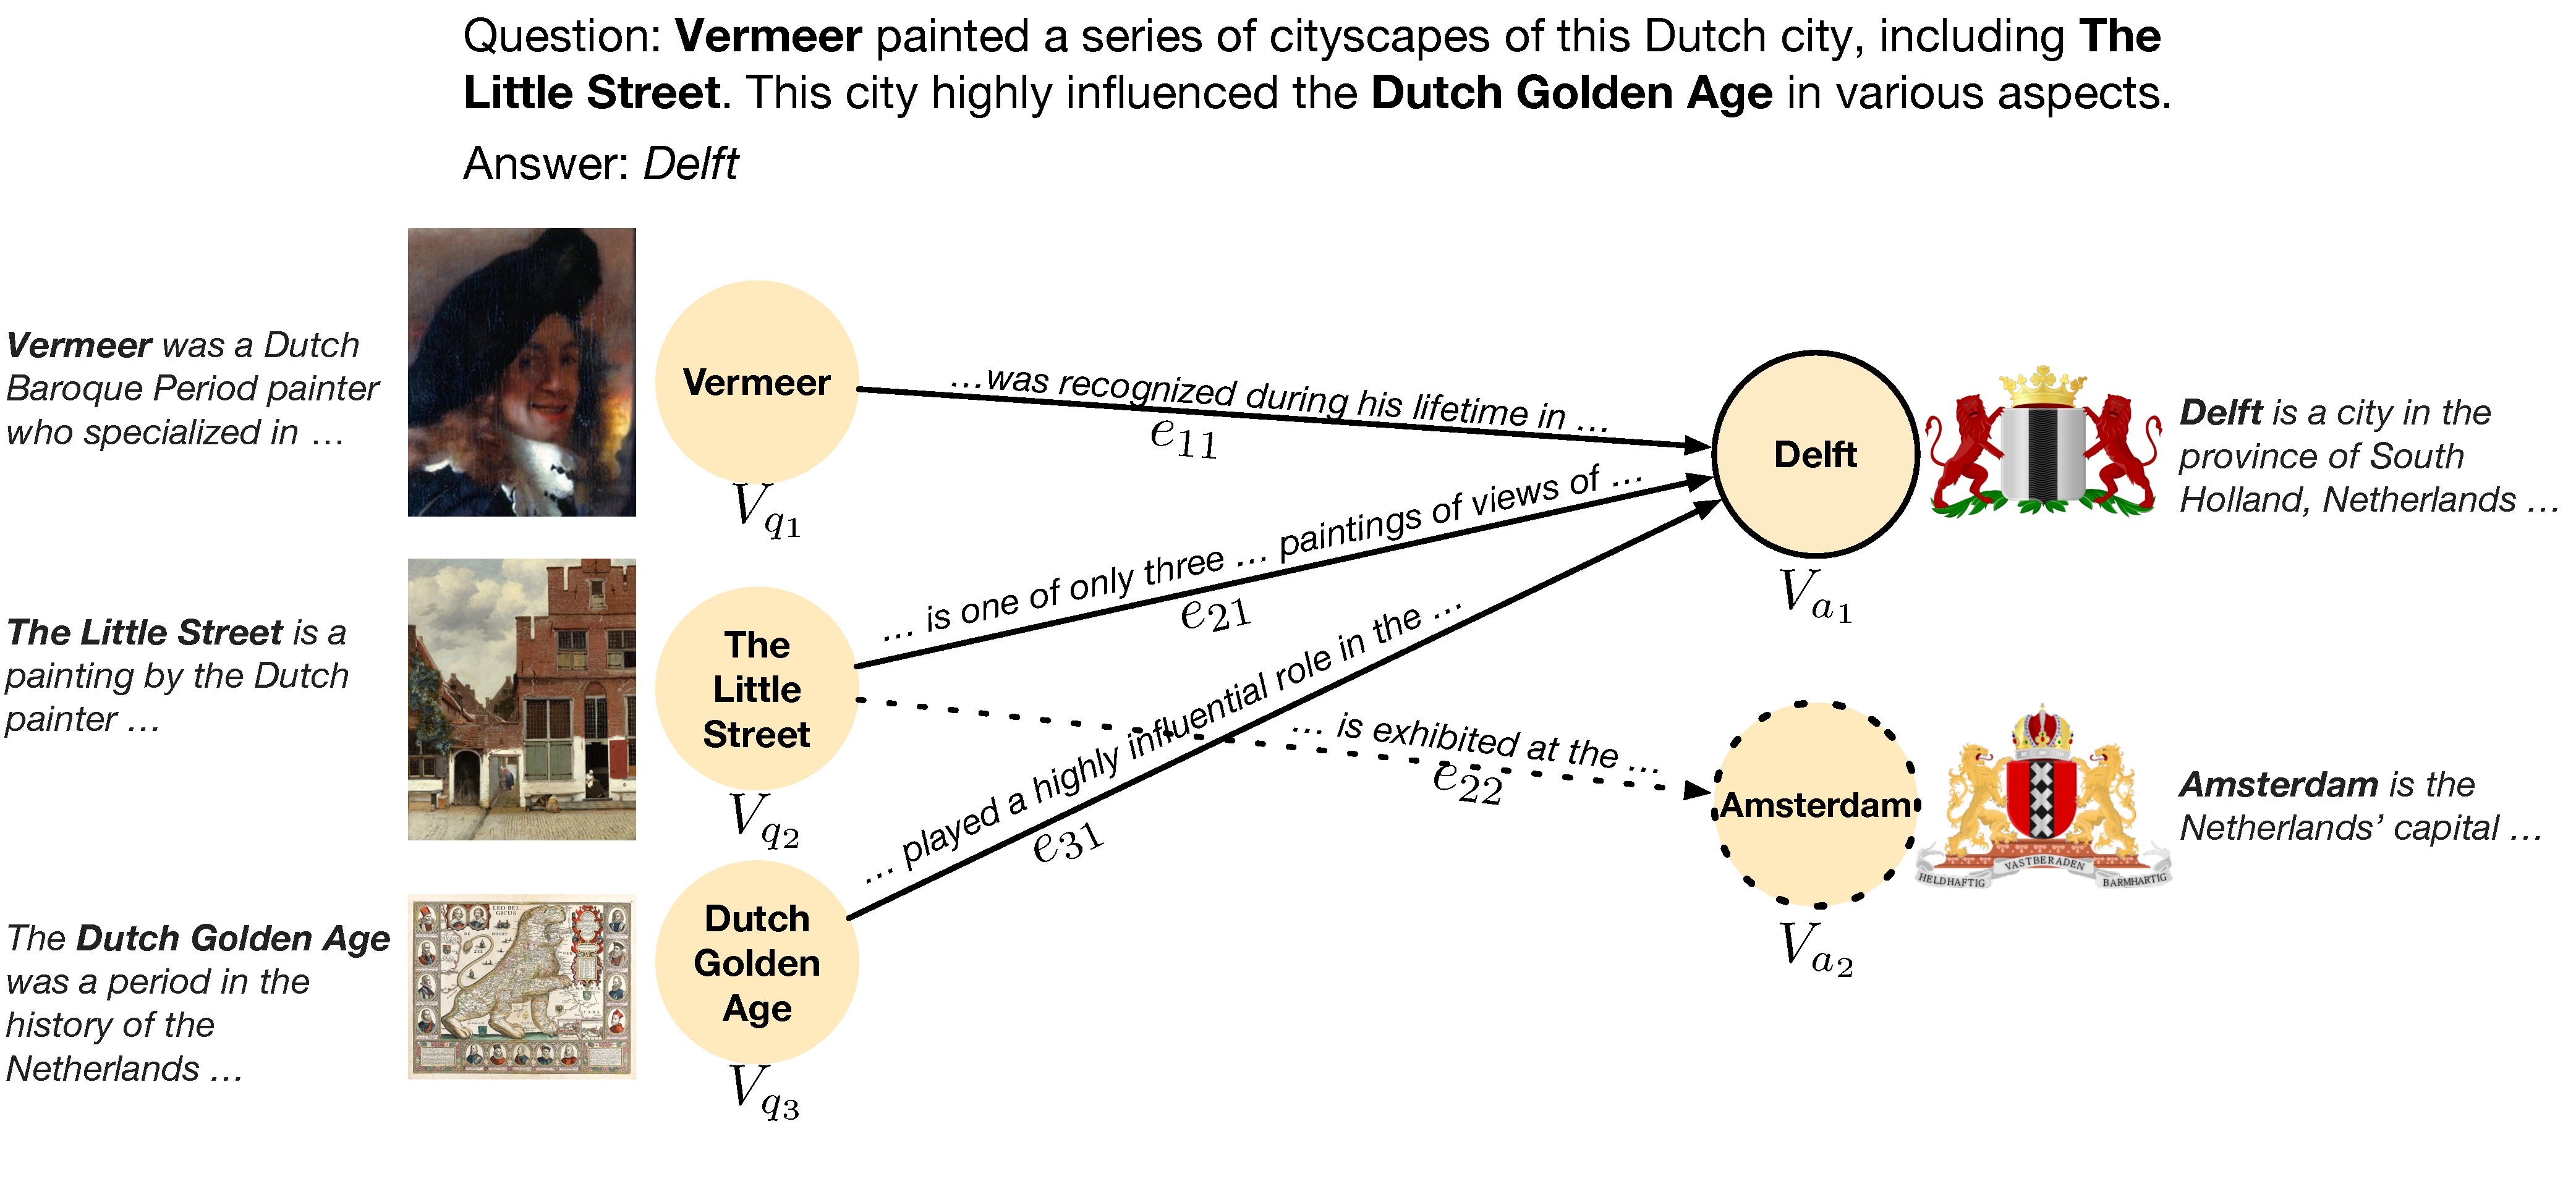
\includegraphics[width=0.9\linewidth]{2020_www_delft/figures/fig_overall.pdf}
    \end{center}
    \caption{An example question grounded free-text knowledge graph in
      \name{}. The graph has both question entity nodes (left side)
      and candidate entity nodes (right side), and use natural
      language sentences from Wikipedia for both nodes and edges.}
    \label{fig:graph}
          %\jbgcomment{Label candidates, question entities, and evidence edges \textbf{in the figure}}
\end{figure*}


Unlike existing knowledge graphs, in which the relations between
entities are well-defined, \name{} leverages informative, diverse, but noisy
relations using a novel graph neural network (\abr{gnn}).
%
Each edge in our graph is associated with multiple sentences that give
explain how entities interact with each other. \name{} uses the \abr{gnn} to distinguish the 
useful evidence information from unrelated text and aggregates
multiple evidence from both text and the graph structure to answer the question.
%
%To find the most useful sentences, the \abr{gnn}
%focuses on the text which is most similar to (and thus can resolve)
%the question text.
%
%Finally, the network selects an answer to the question using the
%accumulated evidence for each of the candidates.

We evaluate \name{} on three question answering
datasets: \qblink{},  \qanta{}, and \triviaqa{}.
%
\name{} outperforms machine reading based model~\cite{chen2017reading},
\abr{bert}-based answer ranking~\cite{devlin2018bert}, and a \abr{bert}-based memory
network approach~\cite{weston2014memory} that uses the same evidence
but no graph structure, with significant margins.
%
Its accuracy improves on more complex questions and when dense
evidence is available, while \abr{mr} cannot take advantage of
additional evidence.

Ablation reveals the importance of each model component: node
representation, edge representation, and evidence combination.
Our graph visualization and case studies further illustrate that our
model could aggregate multiple pieces of evidence to make a more
reliable prediction.\footnote{The code, data, full free-text knowledge graph, and question grounded subgraph
is at \url{delft.qanta.org}. }
